% !TEX root = ../featureselection.tex
The visualization research community has usually focused on developing techniques and systems to support the analysis of data sets, with limited analysis of the relationship between data sets and the construction of models on top of them. However, there are a growing number of data scientists interested in more than just interpreting their data: they want to understand their data and predictive probabilities associated with them. Providing visual support for this kind of task has become important as many existing applications on the market and in scientific settings need to solve problems that are predictive in nature, \eg, prediction of customer behavior, diseases, drug effectiveness.

Predictive modeling is defined as the process of developing a mathematical tool or model that generates an accurate prediction \cite{kuhn2013applied}. However, building an accurate predictive model is far from trivial. First, modelers must construct cohorts, or distinct groups, to divide their data sets into cases and controls. Then, they must use a feature construction technique to define the feature vector. Next, they must define the parameters for cross-validation to ensure the results are statistically valid and robust. Then, they need to choose a feature selection algorithm to extract the informative features and include them in a model. And finally, they need to choose a classifier to evaluate the predictiveness of the model. For each of these decisions, there are a variety of techniques for cohort construction, feature construction, cross-validation, features selection, and classification to choose from, and there are currently no systematic guidelines to decide which algorithms are most appropriate for which types of data sets. Making the wrong choices can cause predictive models to fail. Kuhn and John argue that many predictive models fail because, ``predictive modelers often only explore relatively few models when searching for predictive relationships [...] due to either modeler's preference for, or knowledge of, or expertise in, only a few models or the lack of available software that would enable them to explore a wide range of techniques" \cite{kuhn2013applied}. We use these current limitations as motivation to research how visual analytics may improve the process of predictive modeling.

\begin{figure}[t]
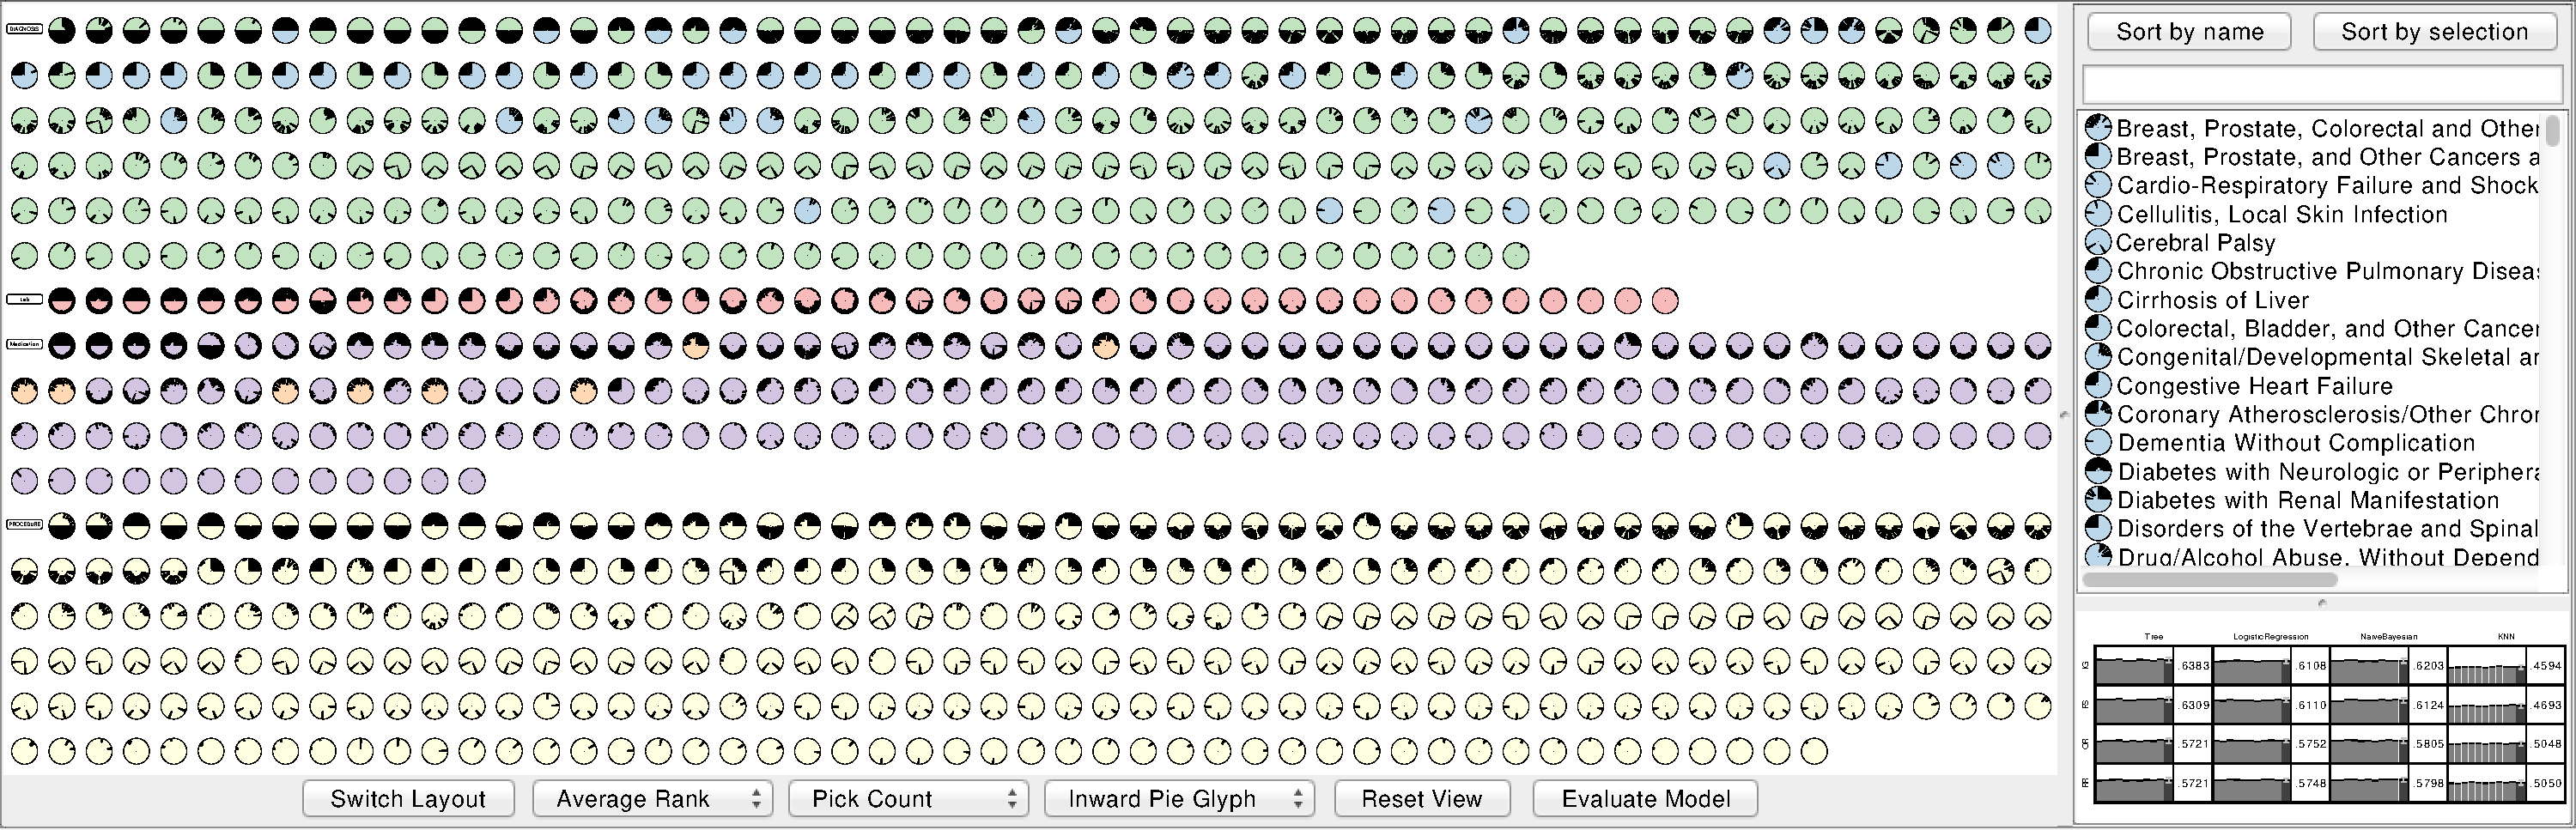
\includegraphics[width=\textwidth]{infuse/teaser}
\caption[Overview of \infuse.]{
An overview of \infuse, a visual analytics tool that supports users to understand the predictive power of features in their models.  Each feature is ranked by various feature selection algorithms, and the ranking information is visualized in each of the three views within the system.  On the left, the Feature View provides a way to visualize an overview of all features according to their rank using a variety of layouts.  On the top-right, the List View provides a sorted list of all features, useful for selections.  On the bottom-right, the Classifier View provides access to the quality scores of each model.  Each of the views are coordinated, and users can brush between all three views.
}
\label{fig:teaser}
\end{figure}

Our proposed research focuses on an important step in the predictive modeling pipeline: feature selection. When data is high-dimensional, feature selection algorithms are often used to remove non-informative features from models. Again, the analyst is confronted with the decision of which feature selection algorithm to utilize, and even if the analyst decides to try out multiple types, the algorithmic output is often not amenable to user interpretation. This limits the ability for users to utilize their domain expertise during the modeling process. To improve on this limitation, we developed \infuse (INteractive FeatUre SElection), a novel visual analytics system designed to help analysts understand how predictive features are being ranked across feature selection algorithms, cross-validation folds, and classifiers. We describe the tasks associated to the feature selection and understanding process and provide a design rationale for our solution. We also demonstrate, through case studies, how the system can lead to important insights for clinical researchers predicting patient outcomes from electronic medical records.

Concretely, our contributions include:

\begin{itemize}
\item A design and implementation of a predictive modeling exploration system,
\infuse, for understanding how predictive features are being ranked
across feature selection algorithms, cross-validation folds, and classifiers.
\item An Interactive Model Builder, where users can create customized models based on insights reached with \infuse, and then have their results evaluated in comparison to automated methods.
\item A case study of domain experts using
\infuse  to explore predictive models in electronic health records.
\end{itemize}

\begin{figure}[t]
\centering
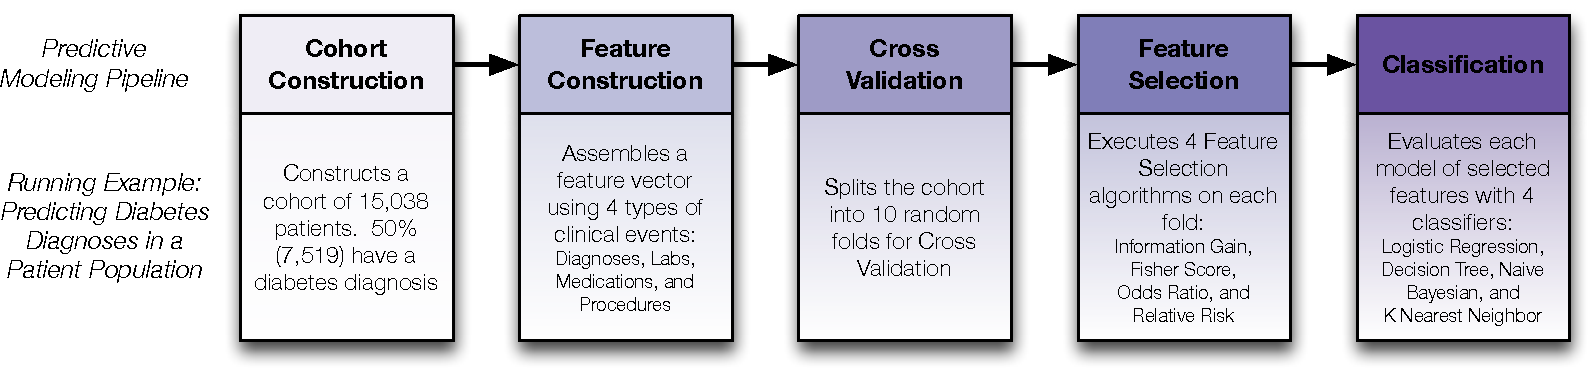
\includegraphics[width=\linewidth]{infuse/pipeline}
\caption[Steps of a typical predictive modeling pipeline.]{Steps of a typical predictive modeling pipeline.  For each step, we provide the details of the running example we use throughout the paper.
}
\label{fig:pipeline}
\end{figure}

% The following text is taken from the PARAMO paper:
% "To develop an accurate and useful predictive model, a research- er generally needs to build and compare many different models as part of the discovery workflow. Each model can be viewed as an instance of the modeling pipeline and consists of a unique combination of the data, algorithms, and/or certain parameter configurations in the task components.
% A number of factors combine to increase the number of models that need to be explored, resulting in a large set of pipelines that have to be processed. First, the volume, variability, and heteroge- neity of EHR data require significant processing in building predic- tive models [10]. Second, there is uncertainty in knowing a priori which feature construction, feature selection, and classification algorithms are most appropriate for the specific target application [27]. As such, composition of an appropriate predictive model re- quires exploring a potentially large space of possible algorithms and parameters and their combinations. Third, for some biomedi- cal applications, the ability to interpret how the model works is just as, if not more, important than the accuracy of the model. Here, it is important to explore a variety of classification algo- rithms (e.g. decision trees, Bayesian networks, and generalized regression models) that produce trained models which can be interpreted by domain experts to verify and validate that the mod- el is clinically meaningful [28]. It is likely that multiple models can have similar performance in terms of prediction accuracy, but may differ significantly in their internal model parameters. By building multiple models, it becomes possible to select ones that have more clinically meaningful interpretations. Fourth, it is critical to statis- tically validate the models to ensure generalizability and accuracy. Cross-validation techniques can help with this endeavor, but can dramatically increase the number of models that need to be built and evaluated.""

\begin{figure}
\centering
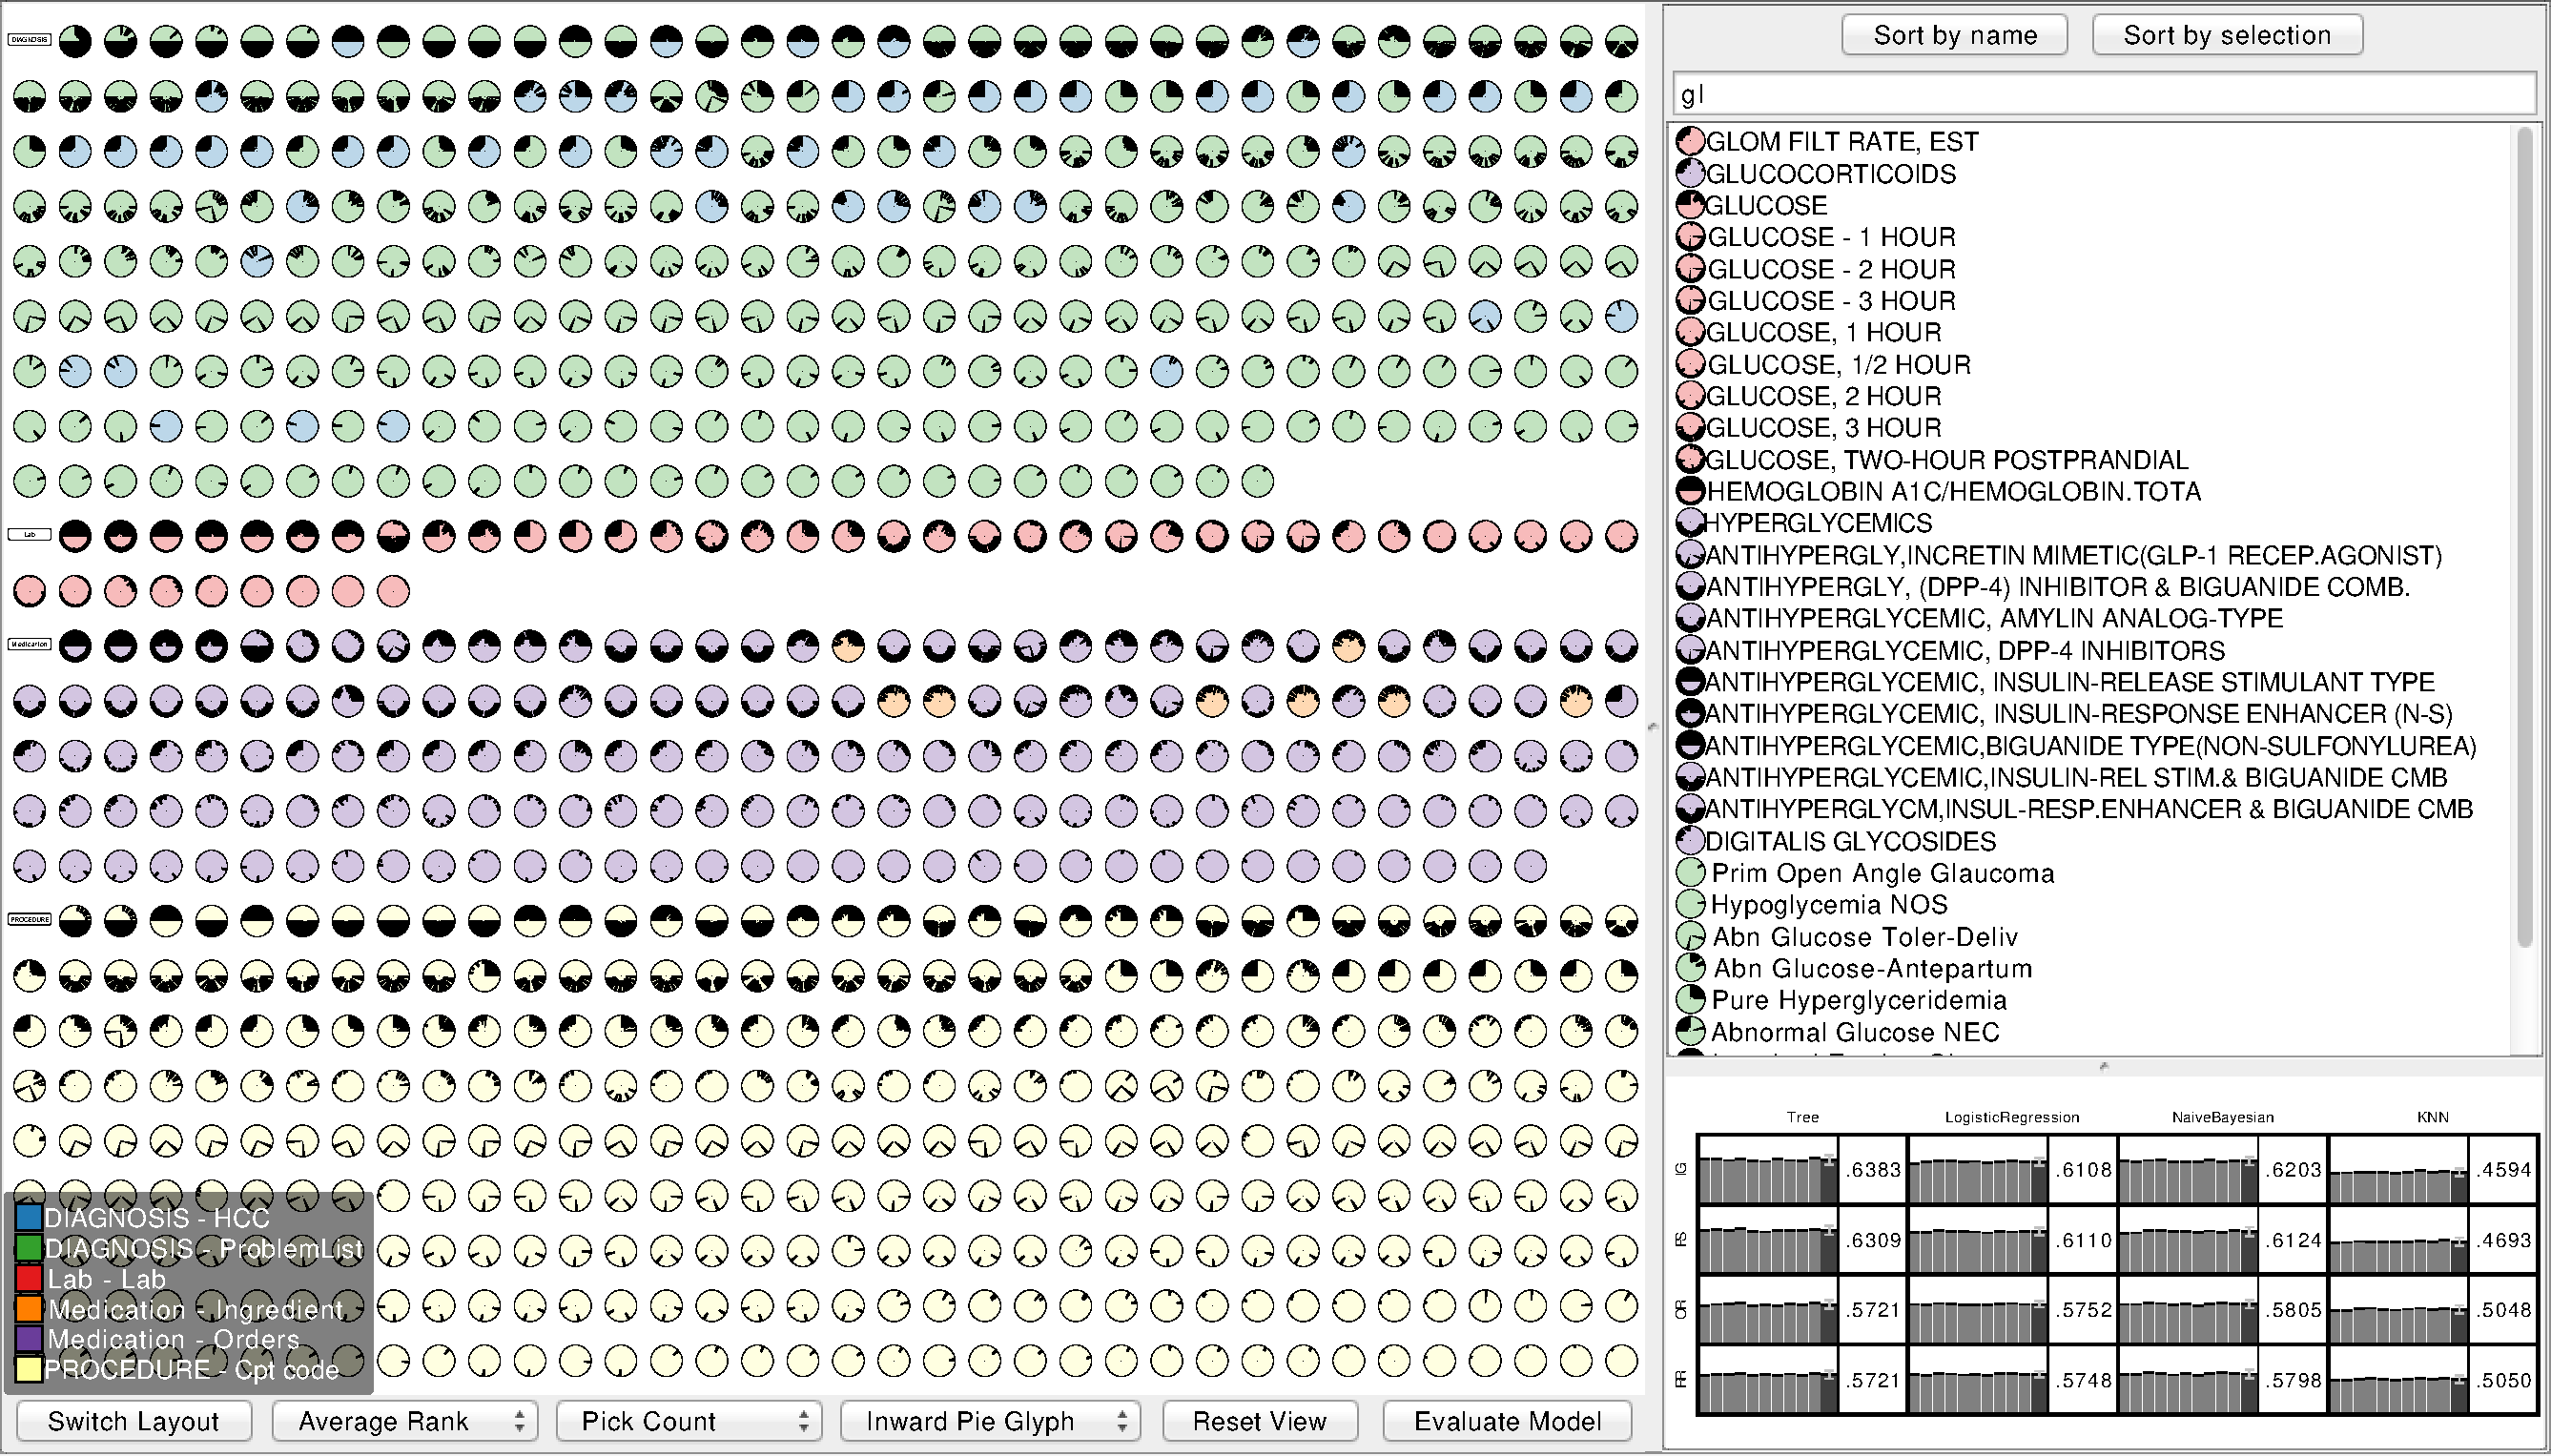
\includegraphics[width=\linewidth]{infuse/system}
\caption[Breakdown of the user interface of \infuse.]{
An overview of \infuse, a system for interactive feature selection.  On the left, the Feature View provides a way to visualize an overview of all features grouped by type and then sorted by importance.  The color key for the feature types and subtypes are shown at the bottom.  The buttons and combo boxes at the bottom can be used to switch layouts and define the axes of the scatterplot view shown in
Figure~\ref{fig:scatter}.  On the top-right, the List View provides a sorted list of all features, useful for selections.
This list can be filtered using the search box above. Currently only features containing the term ``gl" are shown.
The remaining features are sorted by the number and position
of the search term occurrences.
On the bottom-right, the Classifier View (Figure~\ref{fig:classifier}) provides access to the quality scores of each model.  Users can also select features and build custom models with the Interactive Model Builder.
}
\label{fig:system}
\end{figure}
